\chapter{RVfpga}
\label{chapter:rvfpga}
\section{Baseline SoC: RVfpgaNexys}
In chapter \ref{chapter:RISC-V}, after analyzing several different RISC-V based SoCs, the SweRVolf SoC was chosen as the baseline SoC for this thesis. RVfpgaNexys \cite{} is an extended version of SweRVolf targeted to the Nexys A7 board. The extended SweRVolf, or SweRVolfX, adds 4 peripherals to SweRVolf: a GPIO, a PTC, an additional SPI, and a controller for the 8 digit 7-Segment Displays.

\begin{figure}[h]
    \centering
    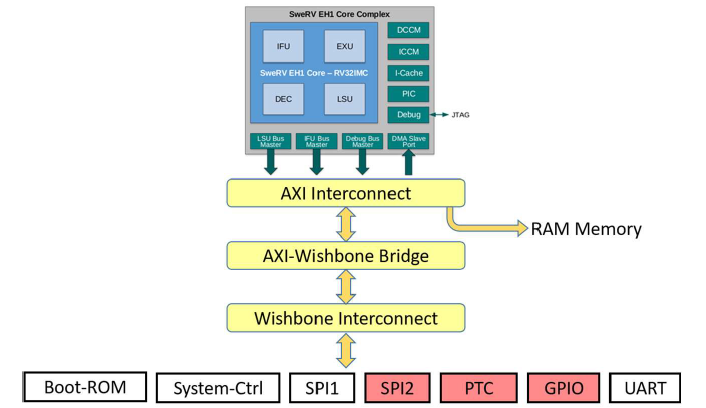
\includegraphics[scale=0.7]{Figures/SweRVolfX.png}
    \caption{SweRVolfX block diagram from Imagination Technologies}
    \label{fig:SweRVolfX}
\end{figure}

Figure \ref{fig:SweRVolfX} shows the block diagram of the SweRVolfX SoC. The SoC utilizes the SweRV EH1 Core Complex from Western DIgital with a 32-bit (RV32ICM) core. The SweRVolf SoC includes a Boot ROM, UART, a System Controller and an SPI controller. The peripherals use a Wishbone bus, however the SweRV EH1 Core uses an AXI bus, so the SoC also includes a AXI to Wishbone bridge.

\begin{figure}[H]
    \centering
    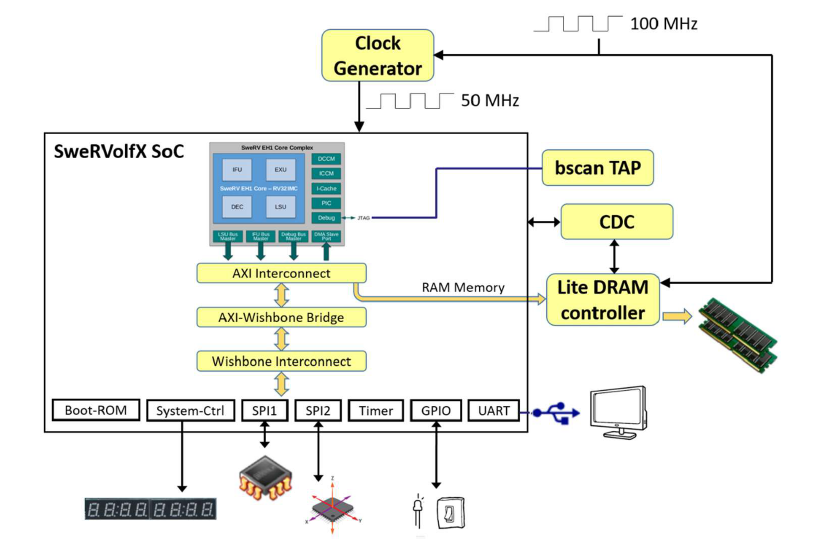
\includegraphics[scale=0.7]{Figures/RVfpgaNexys.png}
    \caption{RVfpgaNexys block diagram from Imagination Technologies}
    \label{fig:RVfpgaNexys}
\end{figure}

Figure \ref{fig:RVfpgaNexys} has a block diagram that shows how the SweRVolfX SoC and the Nexys A7 board interact with each other.



\section{AXI Interconnect}


\section{Hardware Accelerator}


\section{Conclusions}